\documentclass[12pt]{article}
\usepackage{amsmath}
\usepackage{float}
\usepackage{algorithm}
\usepackage{amssymb}
\usepackage{graphicx}
\usepackage{hyperref}
\usepackage{cleveref}
\usepackage[most]{tcolorbox}
\usepackage[utf8]{inputenc}
\usepackage{tikz}
\usepackage{pstricks-add}
\usepackage{centernot}
\usepackage{algpseudocode}
\usepackage{enumerate}
\usepackage{MnSymbol}
\usepackage{mathtools}
\usepackage{subcaption}
\usepackage{geometry}
 \geometry{
 a4paper,
 total={170mm,257mm},
 left=20mm,
 top=20mm,
 }
\DeclarePairedDelimiter\ceil{\lceil}{\rceil}
\DeclarePairedDelimiter\floor{\lfloor}{\rfloor}
\DeclarePairedDelimiter\abs{\left|}{\right|}
\DeclareMathOperator{\arcsec}{arcsec}
\DeclareMathOperator{\arccot}{arccot}
\DeclareMathOperator{\arccsc}{arccsc}
\hypersetup{
    colorlinks=false,
    pdfborder={0 0 0},
}
\newcommand\tab[1][1cm]{\hspace*{#1}}
\newtheorem{theorem}{Theorem}
\newtheorem{corollary}{Corollary}
\usetikzlibrary{arrows,calc}
\title{MAT 1001: Calculus I}
\author{Alfonsus Rodriques Rendy}
\date{2021-12-12}

\begin{document}
\begin{center}
    \hspace*{-0.5cm}
    \framebox{
    \begin{minipage}{1\linewidth}
        \textbf{MAT1001 Calculus I} \\
        \vspace{-0.8cm}
        \begin{center}
            \huge{Lecture 26 - 27 : First Order Differential Equations} 
            \\
            \vspace{0.5cm}
            \normalsize \textit{Lecture by Dr. Arjan Abeynaike} \\
            \vspace{0.3cm}
            \text{Scribe by Alfonsus Rodriques Rendy} \\
            \textrm{Nov 9, 2021 - Dec 14, 2021}
        \end{center}
    \end{minipage}}
\end{center}

\section{Growth Model}
\subsection{Malthusian Growth Model}
Malthusian growth model is based on the assumption that the population grows at 
a rate proportional to the size of the population. Lat $P(t)$ represents the population at time $t$, then
\[
    \frac{dP}{dt} = kP 
\]
for some constant $k$

\subsection{Logistic Growth Model}
Since population is not likely to grow indefinitely due to limited resources and other constaints, a new model is created. The new more practical
model would assume that initially $P$ grows proportionally with $P$ and the growth will decrease as $P$ gets closer to a certain carrying capacity $M$.
\[
    k = r(M - P)
\]
where $r > 0$ is a constnat. then in this case 
\[
    \frac{dP}{dt} = kP = r(M - P)P = rPM(1 - \frac{P}{M})
\]

if we set a constant $K = rM$ then
\[
    \frac{dP}{dt} = KP(1 - \frac{P}{M})
\]
\section{Differential Equations}
\subsection{Definition}
A \textbf{first-order differential equation} (D.E.) is an equation of the form 
\[
    \frac{dy}{dx} = F(x,y)
\]
where $y$ is the dependent variable and $x$ is the independent variable. \\

\noindent
A solution to a first-order differential equation is a function $y = y(x)$ defined on some interval $I$ such that 
\[
    y'(x) = F(x, y(x)) \textrm{\tab} \forall \, x \in I
\]
A general solution to a first-order differential equation is the collection of all solutions to the equation.

\noindent 
A \textbf{first-order initial value problem (IVP)} is a first-order differential equation with an initial value condition:
\begin{align*} 
    \begin{cases} 
    \frac{dy}{dx} = F(x, y) \\
    y(x_0) = y_0
    \end{cases} 
\end{align*}
A particular solution is a solution that satisties the IVP.

\paragraph{Example} Show that $y = (x^3 + 8)^{1/3}$ is a particular solution to the IVP
\[
    y' = \frac{x^2}{y^2} \textrm{\tab} y(0) = 2
\]

\[
    y' = \frac{1}{3}(x^3 + 8)^{ - \frac{2}{3}} (3x^2) = \frac{x^2}{(x^2 + 9)^{\frac{2}{3}}} = \frac{x^2}{y^2}
\]
\[
    y(0) = (0 + 8)^\frac{1}{3} = 2
\]

\subsection{Slope Fields}
Given a D.E. we can graph the solutions using slope fields. Suppose 
$y = f(x)$ is a solution satisfying $f(x_0) = y_0$ then:
\begin{itemize} 
     \item The graph passes through $(x_0, y_0)$ 
     \item $f'(x_0) = F(x_0, y_0)$
     \item The slope of the tangent line to $y = f(x)$ = $F(x_0, y_0)$
\end{itemize}
So to sketch the solution curves first plot may points on the plance with each plotted point $(x_0, y_0)$ have a short 
line segment with slope $F(x_0, y_0)$.

\paragraph{Example} Sketch the slope field for
\[
    \frac{dy}{dx} = y - x
\]

\begin{figure}[H]
     \centering
     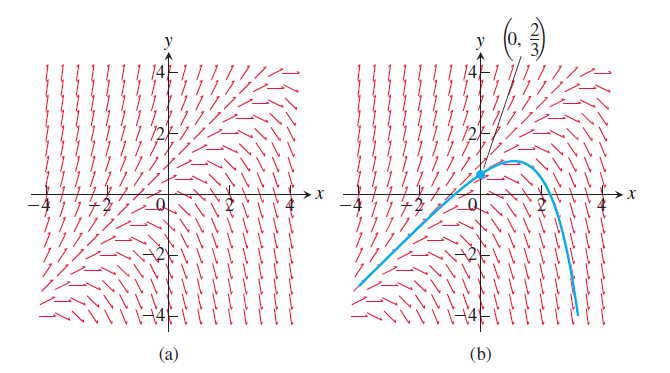
\includegraphics[width = 0.7\linewidth]{Images/slope fields.png}
     \caption{The slope fields for $dy/dx = y - x$}
\end{figure}

\subsection{Euler's Method}
Given an IVP $\frac{dy}{dx} = F(x, y)$ with $y(x_0) = y_0$, suppose we want to find $y(s)$ with $s = x_0 + 1$
\begin{itemize} 
    \item If we can solve $y = y(x)$ explicitly, then we can find $y(s)$
    \item Otherwise numerical methods are required, such as Euler's method
\end{itemize}
The main idea is to start with $(x_0, y_0)$ and approximate the solution curve $y = y(x)$ by generating a sequence of points 
$(x_0, y_0), (x_1, y_1), (x_2, y_2)$ ... using tangent line approximation.
Let $(x_0, y_0)$ be the starting point. Pick a small $\Delta x$, then 
\begin{align*} 
    \textrm{set }\begin{cases} 
        x_1 = x_0 + \Delta x \\ 
        y_1 = y_0 + F(x_0, y_0)\Delta x
    \end{cases} 
\end{align*}
$y_1$ is approximation of $y(x_0 + \Delta x)$, which is $y(x_1)$. And repeat the same procedure until $x_n$.
\begin{figure}[H]
     \centering
     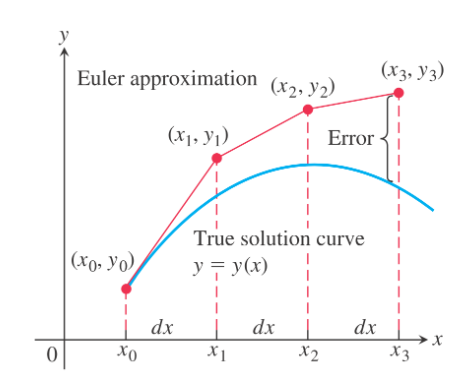
\includegraphics[width = 0.4 \linewidth]{Images/euler method.png}
     \caption{Illustration of Euler's method}
\end{figure}

\paragraph{Example} Given $y' = 1 + y$ and $y(0) = 1$, approximate $y(0.3)$ with $\Delta x = 0.1$
\begin{align*} 
     x_0 = 0 \quad y_0 = 1 \\
     x_1 = 0.1 \quad y_1 = 1 + (1 + 1)(0.1) = 1.2 \\
     x_2 = 0.2 \quad y_1 = 1.2 + (1 + 1.2)(0.1) = 1.42 \\
     x_3 = 0.3 \quad y_1 = 1.42 + (1 + 1.42)(0.1) = 1.662 \\
\end{align*}
Hence
\[
    y(0.3) = y(x_3) \approx y_3 = 1.662
\]
The exact solution is:
\[
    v(x) = e^{\int ( 1) \, dx} = e^{ -x}
\]
\[
    y = \frac{1}{e^{ - x}} \int e^{ - x} \, dx = e^x( -e^{- x} + C) = - 1 + Ce^x
\]
\[
    y(0) = 1 \Rightarrow 1 = - 1 + C \Rightarrow C = 2
\]
Hence
\[
    y(0.3) = - 1 + 2e^{0.3} \approx 1.6997
\]
\section{Solving Methods}
\subsection{Separable Equations}
\paragraph{Definition}
A differential equation of the form 
\[
    \frac{dy}{dx} = g(x)f(y)
\]
is said to be separable

\paragraph{Example} $y' = e^xe^y$ is separable and $y' = e^x + e^y$ is not separable

\noindent
Suppose that $y' = g(x)f(y)$ and $f$ is not a zero function then
\[
    \frac{1}{f(y)} y' = g(x) \Rightarrow \int \frac{1}{f(y)} \, dy = \int g(x) \, dx
\]

\paragraph{Solving Separable Function} If $\frac{dy}{dx} = g(x)f(y)$, by letting $h(y) = \frac{1}{f'(y)}$ we have
\[
    \frac{dy}{dx} = \frac{g(x)}{h(y)} = \int g(x) \, dx = \int h(y) \, dy
\]

\paragraph{Example 1} Solve $y' = e^{x + y}$
\begin{align*} 
    \frac{dy}{dx} &= e^{x + y} = e^x e^y \\
    \int \frac{1}{e^y} \, dy &= \int e^x dx \\
    - e^{ - y} + C_1 &= e^x + C_2 \\
    - e^{-y} &= e^x + C_2 - C_1 \\
    y &= - \ln{- e^x + C} \textrm{\tab} C = C_2 - C_1
\end{align*}

\paragraph{Example 2} Solve $y' = x^2y$ \\
Suppose $y \neq 0$ for some $x$ then 
\begin{align*} 
    \frac{dy}{dx} &= x^2y \\
    \int \frac{1}{y} \, dy &= \int x^2 \, dx \\
    \ln |y|& = \frac{1}{3} x^3 + K \\
    |y| &= e^Ke^{\frac{1}{3}x^3} \\
    y &= \pm e^Ke^{\frac{1}{3}x^3} \\
    y &= Ce^{\frac{1}{3}x^3} \textrm{\tab} C = \pm e^K
\end{align*}
Since zero function is also a solution so, the general solution is 
\[
    y = Ce^{\frac{1}{3}x^3} \textrm{\tab} C \in \mathbb{R}
\]

\paragraph{Example 3} Solve the IVP: $y' = \left( \frac{x}{y} \right)^2$, $y(0) = 2$ \\
\begin{align*} 
    \frac{dy}{dx} &= \frac{x^2}{y^2} \\
    \int y^2 \, dy &= \int x^2 \, dx \\
    \frac{1}{3} y^3 &= \frac{1}{3}x^3 + K \\
    y^3 &= x^3 + 3K \\
    y &= (x^3 + 3K)^{\frac{1}{3}}
\end{align*}
Since $y(0) = 2$:
\[
    2 = (0 + 3K)^\frac{1}{3} \Rightarrow 3K = 8
\]
The particular solution is:
\[
    y = (x^3 + 8)^{\frac{1}{3}}
\]
\subsection{Linear Equations}
\paragraph{Definition} A first-order linear differential equation is an equation of the form
\[
    \frac{dy}{dx} = P(x)y = Q(x)
\]
It is linear because if $\frac{dy}{dx} = F(x, y)$, then 
\[
    F(x, y) = - P(x)y + Q(x)
\]
which is linear in $y$

\paragraph{Intuition} Consider solving
\[
    y' + \frac{y}{x} = 2 \textrm{\tab} x > 0
\]
Multiply both sides with $x$:
\begin{align*} 
    xy' + y &= 2x \\
    (xy)' &= 2x \\
    xy &= x^2 + C \\
    y &= x + \frac{C}{x} \textrm{\tab} C \in \mathbb{R}
\end{align*}

\noindent
Consider solving
\[
    y' + P(x)y = Q(x)
\]
Consider multiplying both sides by $v(x)$ with $v(x)$ is not a zero function:
\[
    v(x)y' + v(x)P(x)y = v(x)Q(x)
\] 

\noindent
If we can choose $v(x)$ such that $v(x)y' + v(x)P(x)y = (v(x)y)'$ then 
\begin{align*} 
    (v(x)y)' &= v(x)Q(x) \\
    \int (v(x)y)' \, dx &= \int v(x)Q(x) \, dx\\
    v(x)y &= \int v(x)Q(x) \, dx \\
    y &= \frac{1}{v(x)} \int v(x)Q(x) \,dx
\end{align*}

\paragraph{Definition: Integrating Factor} Any function $v(x)$ that satisfies 
\[
    \frac{d(v(x)y)}{dx} = v(x) \left(\frac{dy}{dx} + P(x)y \right) 
\]
is called an integrating factor

\begin{align*} 
    (v(x)y)' &= v(x)y' + v(x)P(x)y \\
    v(x)y' + v'(x)y &= v(x)y' + v(x)P(x)y \\
    v'(x)y &= v(x)P(x)y \\
    v'(x) &= v(x)P(x)
\end{align*}

Let $v = v(x)$ then
\begin{align*} 
     \frac{dv}{dx} &= v P(x) \\
    \int \frac{1}{v} \, dv &= \int P(x)\, dx\, \\
    \ln |v| &= \int P(x) \, dx \\
    v &= \pm e^{\int P(x)\, dx}
\end{align*}
Since we only need one integrating factor, then we can choose the positive one with
$\int P(x) \, dx$ to be any particular antiderivative of $P(x)$, then 
\[
    v = e^{\int P(x) \, dx}
\]

\paragraph{Solving Linear D.E.} To solve $y' + P(x)y = Q(x)$, let $v(x) = e^{\int P(x)\, dx}$ where $\int P(x) \, dx$ is any antiderivative of $P(x)$. 
The general solution is given by 
\[
    y = \frac{1}{v(x)} \int v(x)Q(x)\, dx
\]

\paragraph{Example 1} Solve the IVP $xy' + 2y = x^2 - x + 1$ with $x > 0$, $y(1) = \frac{1}{2}$
\[
    y' + \frac{2}{x}y = x - 1 + \frac{1}{x}
\]
Integrating Factor:
\[
    v(x) = e^{\int \frac{2}{x} \, dx} = e^{2\ln x} = x^2
\]
General Solution:
\begin{align*} 
    y &= \frac{1}{x^2} \int x^2 \left( x - 1 + \frac{1}{x}\right) \, dx \\
    y &= \frac{1}{x^2} \int (x^3 - x^2 + x) \, dx \\
    y &= \frac{1}{x^2} \left(\frac{1}{4}x^{4} - \frac{1}{3}x^3 + \frac{1}{2}x^2 + C \right) \\
\end{align*}
Find C:
\[
    y(1) = \frac{1}{2} \Rightarrow \frac{1}{2} = \frac{1}{4} - \frac{1}{3} + \frac{1}{2} + C \Rightarrow C = \frac{1}{12}
\]
Particular Solution:
\[
    y = \frac{1}{4}x^2 - \frac{1}{3}x + \frac{1}{2} + \frac{1}{12x^2}
\]
\paragraph{Example 2} Solve the D.E. $\cos(x)y' + \sin(x)y = 2\cos^3(x)\sin(x) - 1$, $0 \leq x < \frac{\pi}{2}$
\[
    y' + \tan (x)y = 2\cos^2 (x)\sin (x) - \sec (x)
\]
Integrating Factor:
\[
    v(x) = e^{\int P(x) \, dx} = e^{\int \tan x \, dx} = e^{\ln (\sec x)} = \sec x
\]
General Solution:
\begin{align*} 
     y &= \cos x \int \sec(x)(2\cos^2(x)\sin(x) - \sec(x)) \, dx \\
     y &= \cos x \int (2\cos(x)\sin(x) - \sec^2(x)) \, dx \\
     y &= \cos x \int (\sin(2x) - \sec^2(x)) \\
     y &= \cos x \left( -\frac{1}{2}\cos(2x) - \tan(x) + C_0 \right) \\
     y &= - \cos x \left(\frac{1}{2}\cos(2x) + \tan(x) + C \right) \\
\end{align*}
\section{Applications}
\subsection{Population Growth Models}
\paragraph{Malthusian Growth Model}
\begin{align*} 
    \frac{dP}{dt} &= kP \\
    \int \frac{1}{kP} dP &= t \\
    \frac{1}{k} \ln P &= t + A \\
    \ln P^{\frac{1}{k}} &= t + A \\
    P^{\frac{1}{k}} = e^{t + A} &= e^Ae^t \\
    P &= e^{kA}e^{kt} \\
    P &= Ce^{kt}
\end{align*}
If $P(0) = P_0$ then $P_0 = Ce^0 = C$. Hence the particular solution is:
\[
    P = P_0e^{kt}
\]
where $P_0$ is the initial population.

\paragraph{Logistic Growth Model}
Let $0 < P < M$ is the carrying capacity
\begin{align*} 
    \frac{dP}{dt} &= kP(1 - \frac{P}{M}) \\
    \frac{dP}{dt} &= \frac{kP(M - P)}{M} \\
    \int \frac{M}{P(M - P)} \, dP &= \int k \, dt \\
    \int \frac{1}{P} \, dP + \int \frac{1}{M - P} \, dP &= kt \\
    \ln P - \ln (M - P) &= kt + A \\
    \ln \left( \frac{P}{M - P}\right) &= kt + A \\
    \frac{P}{M - P} &= e^Ae^{kt} \\
    \frac{M - P}{P} &= e^{ - A}e^{ - kt} \\ 
    \frac{M}{P} &= 1 + Ce^{ - kt} \textrm{\tab} C = e^{-A} \\
    P &= \frac{M}{1 + Ce^{ - kt}} \textrm{\tab} C > 0
\end{align*}
If the initial condition is $P(0) = P_0$ then 
\[
    P_0 = \frac{M}{1 + C} \Rightarrow C = \frac{M - P_0}{P_0} 
\]
\paragraph{Properties of logistic function}
\begin{itemize} 
     \item $P$ is increasing with t
     \item $\lim_{t \to \infty} P(t)$ = $M$
     \item $P$ has a point of inflection when $M/2$. Assume this point is $(t_1, M/2)$ then $P$ is concave up on $(-\infty, t_1)$ and concave down on $(t_1, \infty)$
\end{itemize}
\subsection{Mixing Problem}
\paragraph{Example} Consider a container satisfying the following conditions:
\begin{itemize} 
     \item It initially contains $10000 L$ of solution, having 50 kg of salts dissolved in it 
     \item The solution leaks out of the container at a rate 220 L/min
     \item A solution with salt whose concentration is 0.2 kg/L is pumped into the container at a rate of 200 L/min
\end{itemize}
Suppose that the newly added solution is instantly well mixed with the solution that was already in the container. What is the amount of salf in the container
20 minutes after the initial time?

\paragraph{Solution}
Let $y(t)$ = mass of salt $t$ minutes since the beginning, then $y(0) = 50$, what is $y(20)$? 
\begin{align*} 
    \frac{dy}{dt} &= \textrm{rate in - rate out} \\
    &= (200)(0.2) - (220)\frac{y(t)}{V(t)} \\ 
    &= 40 - 220\cdot \frac{y(t)}{10000 - 20t} \\
    &= 40 -\frac{11y(t)}{500 - t} 
\end{align*}
The IVP is:
\begin{align*} 
    \begin{cases} 
    y' = 40 - \frac{11y(t)}{500 - t} \\
    y(0) = 50 
    \end{cases} 
\end{align*}

\[
    y' + \frac{11}{500 - t} y(t) = 40
\]
Integrating Factor:
\[
    v(x) = e^{\int P(t) \, dt} = e^{\int \frac{11}{500 - t} \, dt} = (500 - t)^{ - 11} 
\]
General Solution:
\begin{align*} 
     y &= \frac{1}{v(t)} \int v(t)Q(t) \, dt \\
     &= (500 - t)^{11} \int 40(500 - t)^{11} \, dt \\
     &= (500 - t)^{11} \left( \frac{40}{ - 10} ( - 1) (500 - t)^{ - 10} + C \right)\, \\
     &= 4(500 - t) + C(500 - t)^{11}
\end{align*}
Find C:
\[
    y(0) = 50 \Rightarrow 50 = 2000 + C(500)^{11} \Rightarrow C = - \frac{1950}{500^11}
\]
Particular Solution:
\[
    y(t) =  4(500 - t) - \frac{1950}{500^11}(500 - t)^{11}
\]
After $t = 20$:
\[
    y(20) = 1920 - 1950(\frac{24}{25})^{11} \approx 675.43
\]
\section{Autonomous Equations}
\subsection{Definition}
An autonomous equation is a differential equation of the form:
\[
    \frac{dy}{dx} = f(y)
\]

\paragraph{Example}
\begin{itemize} 
    \item $\frac{dP}{dt} = kP$ is autonomous (Malthusian growth model)
    \item $\frac{dP}{dt} = kP\left( 1- \frac{P}{M} \right)$ is autonomous (Logistic growth model)
\end{itemize}
If we think of $y = y(t)$ as the position of a moving particle on the y-axis at time $t$, then $\frac{dy}{dx} = f(y)$ is stating that
the velocity of the vartical depends only on the position $y$ but not the time $t$.
\subsection{Phase Line Analysis}
Suppose $K$ is a root of $f$, i.e. $f(K) = 0$. Consider the constant function $y = y(x) = K$
\[
    \frac{dy}{dx} = 0 \textrm{\tab} \forall \, x
\]
\[
    f(y) = f(y(x)) = f(K) = 0 \forall \, x
\]
Hence the constant function $y = K$ is a solution to $\frac{dy}{dx} = f(y)$.

\paragraph{Definition}
Given an autonomous equation $\frac{dy}{dx} = f(y)$, for any root $K$ of $f$:
\begin{itemize} 
     \item $K$ is called an \textbf{equilibrium value}
     \item The constant function $y = K$ is called an \textbf{equilibrium solution} to the autonomous equation
\end{itemize}
We can analyse the solutions by drawing all equilibrium points on the y-axis and analysing the signs of derivatives on the intervals
separated by the equilibrium points. We call this \textbf{phase line analysis}

\paragraph{Example}
\[
    \frac{dy}{dx} = y^2 - y - 2 = (y + 1)(y - 2)
\]
The roots (equilibrium values) are -1 and 2. Then phase line analysis:
\[
    \rightarrow( + )\rightarrow[ - 1] \leftarrow( -)\leftarrow [2]\rightarrow ( +)\rightarrow 
\]
\begin{figure}[H]
     \centering
     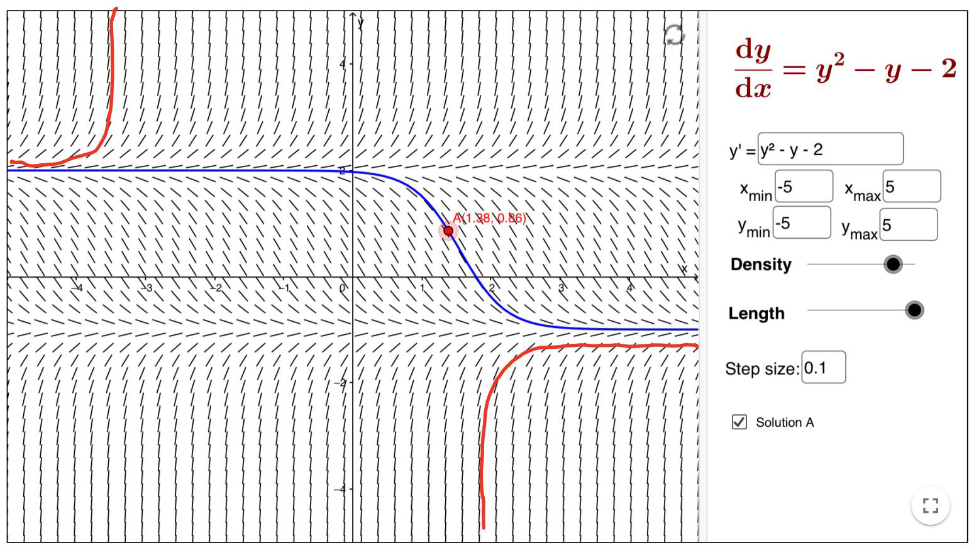
\includegraphics[width = 0.6\linewidth]{Images/phase line analysis.png}
     \caption{Slope fields of $y^2 - y - 2$}
\end{figure}
We can also check the concavity by looking at the second derivative $y'' = (2y-1)y'$
\subsection{Stable and Unstable Equilibrium}
Let $K$ be an equilibrium value of $\frac{dy}{dx} = f(y)$. For any solution $y(x)$ with $y(0)$ near $K$,
$K$ is a stable equilibrium id $y(x)$ moves toward $K$ as $x \to \infty$. Or else, $K$ is an unstable equilibrium.
\begin{figure} 
     \centering
     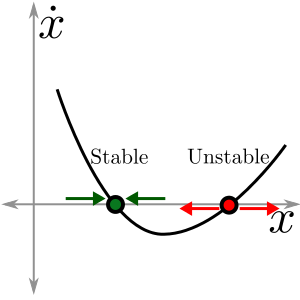
\includegraphics[width = 0.3\linewidth]{Images/equilibrium.png}
     \caption{Stable and Unstable Equilibrium}
\end{figure}

\subsection{Applying on Growth Models}
\paragraph{Phase line analysis on logistics model}
\[
    \frac{dP}{dt} = kP \left( 1 - \frac{P}{M} \right) \quad k > 0 \quad M > 0
\]
Then the equilibrium values are $P = 0$ and $P = M$. Phase line analysis:
\[
    \leftarrow( - )\leftarrow[0] \rightarrow( + )\rightarrow [M]\leftarrow ( -)\leftarrow 
\]
This means that at any given time:
\begin{itemize} 
    \item if $0 < P < M$ then $P$ will increase towards $M$
    \item if $P > M$ then $P$ will decrease towards $M$
    \item if $P = 0$ or $P = M$ then $P$ will stay unchanged     
\end{itemize}
Hence as long as $P(0) > 0$, then $\lim_{t \to \infty} P(t) = M$ \\

\noindent
The malthusian model is unrealistic since $\lim_{t \to \infty} P(t) = \infty$. Hence, the
logistic model is more realistic in that aspect since $\lim_{t \to \infty} P(t) = M$. But it is still
not entirely realistic since even if the population is 1, it will still grow to a population near $M$ instead of facing
extinction. So, a third parameter $m$, minimum population for the population to grow, can be introduced to fix the logistic model.
It's called cubic model
\[
    \frac{dP}{dt} = kP(P - m)(M - P) 
\]
\subsection{Newton's Law of Cooling}
Newton's law of cooling states that the rate of change of the temperatur of an object is proportional
to the difference of temperatures between the object and its surroundings. If $H(t)$ is the temperatur of an object
at time $t$ then $H$ satisfies the differential equation
\[
    \frac{dH}{dt} = k(H - R) \quad k < 0
\]
where $k$ is some negative constants and $R$ is a constant of surrounding temperature.
Then $H = R$ is the equilibrium solution (stable equilibrium)
\begin{figure}[H]
     \centering
     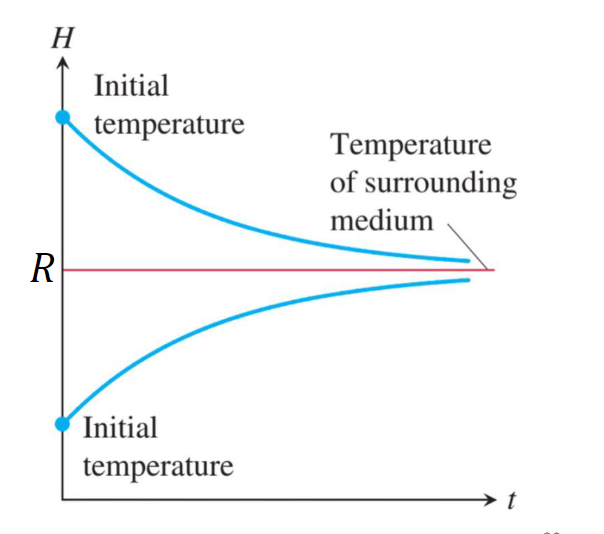
\includegraphics[width = 0.4\linewidth]{Images/newton's law of cooling.png}
\end{figure}
\paragraph{Example}
The body of a murder victim is found at noon in a room with a constant temperature of $20^{\circ}$ C. At noon
the temperature of the body is $35^{\circ}$ C and two hours later the temperature of the body is $33^{\circ}$ C.
Find the temperature $H$ of the body as the function of $t$, the hours since it was found. Assuming that the
body has the normal temperature $37^{\circ}$ C at the time of murder, estimate the time of the murder.

\noindent 
(a) IVP is:
\begin{align*} 
    \begin{cases} 
        \frac{dH}{dt} = k(H - 20) \\
        H(0) = 35
    \end{cases} 
\end{align*}

\begin{align*} 
    \int \frac{1}{H - 20} \, dH &= \int k \, dt \\
    \ln |H - 20| &= kt + C \\
    |H - 20| &= e^{kt + C} = e^Ce^{kt} = Ae^{kt}
\end{align*}
Since $H(0) = 35$, consider $H > 20$:
\begin{align*} 
    H - 20 &= Ae^{kt} \\
    35 - 20 &= 15 = A \\
    H &= 15e^{kt} + 20
\end{align*}
Also, $H(2) = 33$, so
\begin{align*} 
    33 &= 15e^{2k} + 20 \\
    e^{2k} &= \frac{13}{15} \\
    k &= \frac{1}{2} \ln \frac{13}{15}
\end{align*}
Hence:
\[
    H = 15\left(\frac{13}{15}\right)^{\frac{t}{2}} + 20
\]

\noindent
(b) Find $t$ such that
\begin{align*} 
    37 &= 15\left(\frac{13}{15}\right)^{\frac{t}{2}} + 20 \\
    \frac{17}{15} &= \left(\frac{13}{15}\right)^{\frac{t}{2}} \\
    \ln \left( \frac{17}{15} \right) &= \ln \left(\frac{13}{15}\right)^{\frac{t}{2}} \\
    \ln \left( \frac{17}{15} \right) &= \frac{t}{2} \ln \left(\frac{13}{15}\right) \\
    t &= \frac{2 \ln (\frac{17}{15})}{\ln(\frac{13}{15})} \approx\, - - 1.75
\end{align*}
So murder happened approximately 1.75 hours before noon.
\end{document}
